\chapter{System Design, Methodology}\label{chap3}

%##########################################
\vspace*{50 ex}

%##########################################
\paragraph*{Outline:} This chapter presents the following:
\begin{enumerate}
\setlength{\itemsep}{-0.3em}
\item A brief of system design
\item A brief of methodology
\end{enumerate}
\newpage



\section{System Design }


The simplified diagram of the proposed system is
demonstrated in Fig.\ref{img31}. Raspberry pi is the major node
controlling our system. The sensors are being used for
detecting different environmental parameters like particulate
matter, Carbon Monoxide, Carbon Dioxide, Temperature,
Humidity and Pressure. The sensors are connected to Arduino
Board and Raspberry pi is interfaced with Arduino Uno
through USB cable. The data sensed by the sensors are
continuously transmitted through Raspberry pi to the cloud
over the internet because of its good network connectivity.
The sensors DSM501A is a PM sensor whose output is PWM,
used for measuring the particulate matter i.e. smoke and dust
present in our environment, DHT11 and BMP180 are having
digital outputs used for measuring temperature, humidity and
pressure. The sensors, MQ9 (Gas sensor) as well as
MQ135(air quality sensor) are analog sensors used for
measuring Carbon monoxide and carbon dioxide.

\begin{figure}[!ht]
\centering
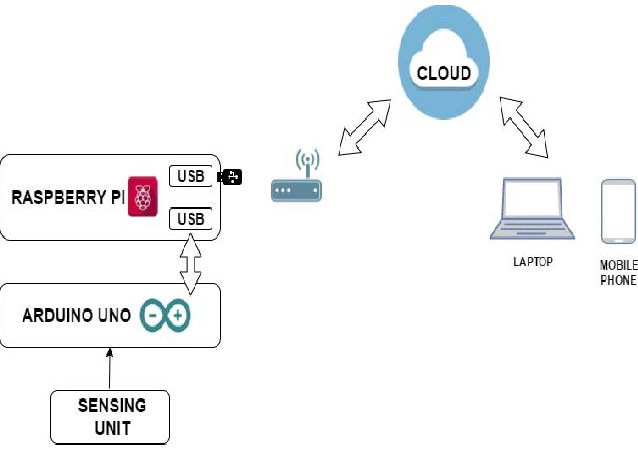
\includegraphics[scale=0.7]{figures/design}
\caption{\label{img31} Simplified diagram of Proposed System}
\end{figure}

Arduino Uno is a low-cost micro-controller board based on
ATMEGA-328P which can be easily interfaced with
Raspberry pi and has a very effective ADC. Since Raspberry
pi 4 has built in Wi-Fi adapter support therefore
Wi-Fi adapter is not used for providing the internet to the
complete system. The light weight protocol MQTT (Message
Queuing Telemetry transport). MQTT plays an important role
in establishing communication between the sensors and the
clients. The client can access the data that is being displayed
on the dashboard by using the device id but the client will be
not able to do any modification to the data received.

\subsection{Raspberry Pi}

Raspberry Pi is a single board computer. It has ARM
Cortex A8 CPU and 1 GB LPDDR4 RAM which makes it a faster and powerful than the previous available models. It has Broadcom
BCM2711, quad-core Cortex-A72 (ARM v8) processor which is running at 1.5 GHz but it can be overclocked. It has 2 × USB 3.0 ports and 2 × USB 2.0 ports, Standard 40-pin GPIO, 2 × micro HDMI ports (up to 4Kp60 supported), 2.4 GHz and 5.0 GHz IEEE 802.11b/g/n/ac wireless LAN, Bluetooth 5.0, 3.5 mm audio jack and
composite video, camera interface (CSI), the display interface
(DSI). It has a separate slot for Micro SD card slot which
is used for storing operating system as well as other software’s
and drivers needed. Raspberry Pi can support different
operating systems such as Raspbian, Windows 10, Ubuntu etc.
Raspbian operating system is used for implementation of
system. Node Red is a visual programming tool for IoT which
is very easy to use. Node Red has an inbuilt library consisting
of thousands of flows and nodes which enable the users to
connect all kind of devices and services. Once the flow is
made it can be deployed and data can be seen on the
dashboard.
\begin{figure}[!ht]
\centering
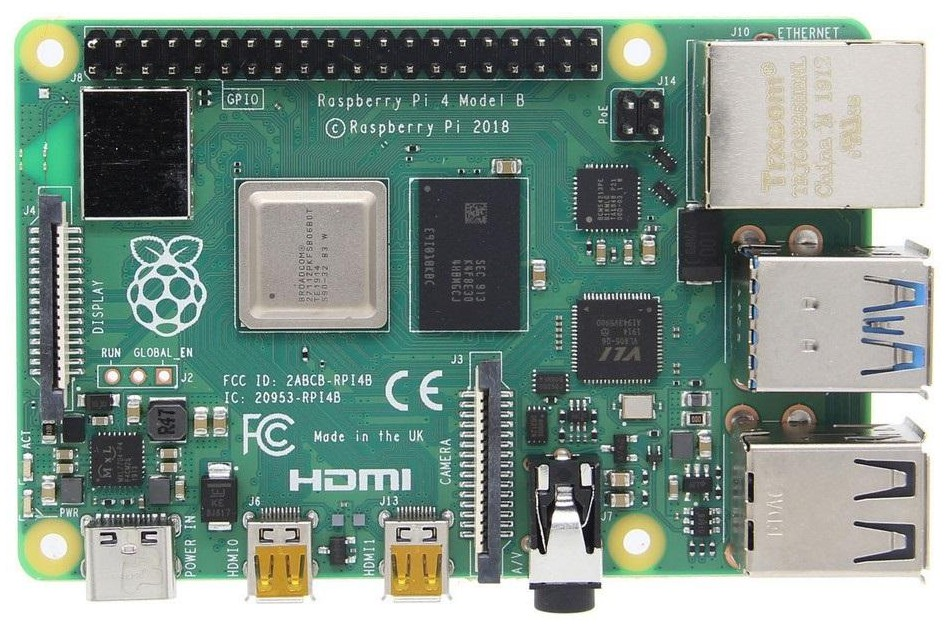
\includegraphics[width=\linewidth]{figures/raspberry.jpg}
\caption{\label{img32} Raspberry Pi 4}
\end{figure}

\begin{figure}[!ht]
\centering
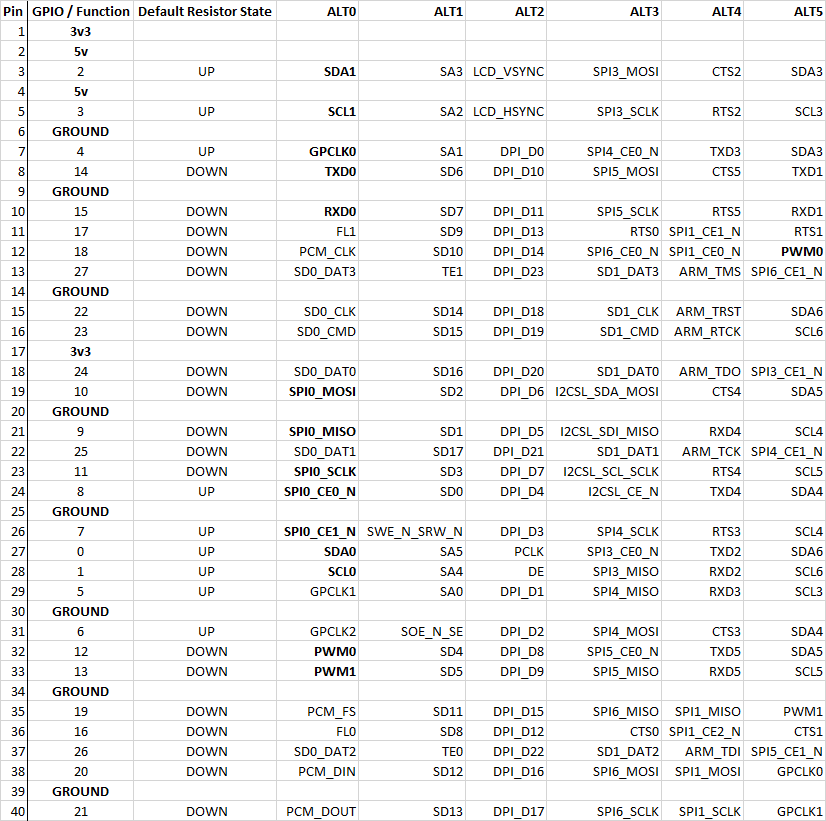
\includegraphics[width=\linewidth]{figures/raspberry-pindiagram.png}
\caption{\label{img33} Pin Diagram of Raspberry Pi 4}
\end{figure}

\begin{figure}[!ht]
\centering
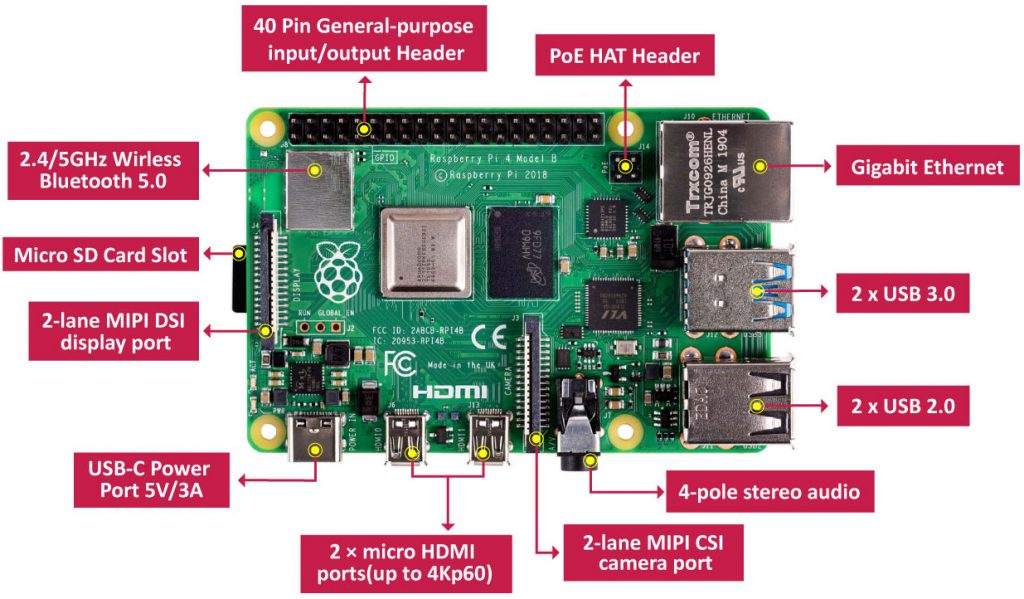
\includegraphics[width=\linewidth]{figures/Raspberry-Pi-pin.jpg}
\caption{\label{img34} Technical Configuration of Raspberry Pi 4}
\end{figure}


\subsection{Arduino UNO}

The Arduino UNO is an open-source microcontroller board based on the Microchip ATmega328P microcontroller and developed by Arduino.cc.The board is equipped with sets of digital and analog input/output (I/O) pins that may be interfaced to various expansion boards (shields) and other circuits. The board has 14 digital I/O pins (six capable of PWM output), 6 analog I/O pins, and is programmable with the Arduino IDE (Integrated Development Environment), via a type B USB cable. It can be powered by the USB cable or by an external 9-volt battery, though it accepts voltages between 7 and 20 volts. It is similar to the Arduino Nano and Leonardo

\begin{figure}[!ht]
\centering
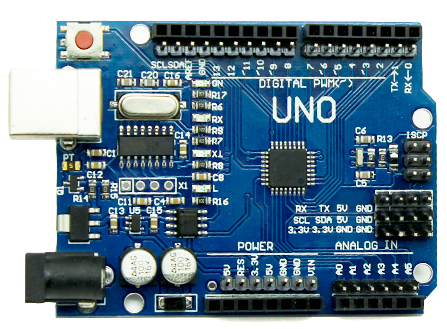
\includegraphics[scale=0.7]{figures/arduino-uno.png}
\caption{\label{img35} Arduino UNO}
\end{figure}

\begin{table}[!ht]
\centering
\begin{tabular}{ |p{5cm}|p{5cm}| }
\hline
\multicolumn{2}{|c|}{Technical specifications} \\
\hline
Microcontroller & ATmega328P\\
Operating Voltage & 5V\\
Input Voltage & 7-12V\\
Input Voltage (limit) & 7-20V\\
Digital I/O Pins & 14\\
PWM Digital I/O Pins & 6\\
Analog Input Pins & 6\\
DC Current per I/O pin & 20mA\\
Dc Current for 3.3V pin & 50mA\\
Flash Memory & 32 KB (ATmega328P)\\
SRAM & 2 KB (ATmega328P)\\
EEPROM & 1KB (ATmega328P)\\
Clock Speed & 16 MHz\\
Length & 68.6 mm\\
Width & 53.4 mm\\
\hline
\end{tabular}
\caption{\label{arduinopin}Arduino UNO Pin Diagram}
\end{table}


\begin{figure}[!ht]
\centering
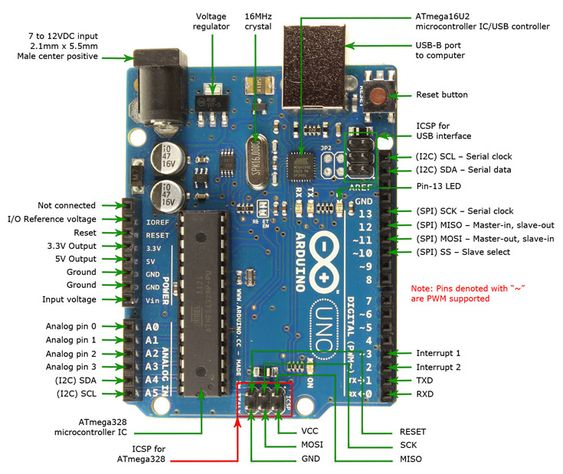
\includegraphics[scale=0.7]{figures/arduino-pin.jpg}
\caption{\label{img36} Technical Configuration of Arduino UNO}
\end{figure}

\subsection{Sensing Unit}

Sensing Unit comprises of five sensors for monitoring the
air pollution. Table 1 shows the technical specifications of the
three air quality sensors, Temperature, Humidity and pressure
sensors. DSM501A is a low-cost dust sensor module has a
very high sensitivity as it can even detect the fine particles
having the diameter greater than 1 micron. MQ9 is highly
sensitive to carbon monoxide / combustible gases. It has a
simple drive circuit and has a prolonged life. With the rise in
concentration of the gases in air, conductivity of the sensors
also increases. MQ135 has wide scope for detection of NH3,
alcohol, CO2, smoke, etc. with a very low response time.
DHT11 is a four-pin, resistive type having digital output
relative humidity and temperature sensor. BMP 180 is a low-
cost sensor used for monitoring barometric air pressure and
can also be used as an altimeter as the pressure changes with
the variations in altitude.

\begin{table}[!ht]
\centering
\begin{tabular}{ |p{4cm}|p{4cm}|p{4cm}|  }
\hline
\multicolumn{3}{|c|}{Sensors List} \\
\hline
Parameter & Operating Voltage & Measuring Range \\
\hline
Particulate Matter & 5 V  & 10 to 10000 ppm\\
Carbon Monoxide & 1.5 V  &10 to 10000 ppm\\
Carbon Dioxide & 5 V  & 10 to 10000 ppm\\
Temperature & 3.3 V  & -40 to +80 degree Celsius\\
Relative Humidity & 3.3 V & 0 to 100 \% RH\\
Pressure & 5 V & 300 to 1100 hPa\\
\hline
\end{tabular}
\caption{\label{sensorsvoltage}Sensors voltage range}
\end{table}


\subsection{Software Architecture}

It involves Node-Red and Integrated Development
Environment.

\subsubsection{Node-RED}

Node-RED is an easy to use, fundamental and an open
source programming tool for IoT applications. It is highly
used visual programming tool which help IoT developers to
integrate Hardware devices, APIs and online services in a very
interesting and creative manner. Built in Library of Node-Red
consist of thousands of flows and nodes that enable the user to
connect all kind of devices and services. Flows can be run at
the edge of network on the hardware like Raspberry pi or in
the cloud since node-red runtime includes node.js. Node-Red
provides a simple click mechanism to deploy the flows by the
IoT developers to a light weight runtime environment.

\subsubsection{Integrated Development Environment}

Arduino programs can be written in any programming
language that has a complier for a conversion of program code
into the binary code. IDE is platform independent acting as the
base for Arduino hardware. It is a very powerful for
programmers, project development professionals and
researchers to develop various Arduino projects employing
different kind of sensors. Arduino IDE is an open source
design/ software which has originated from the integrated
development environment for the languages processing and
wiring projects. As IDE is platform independent, it can run on
Windows, Linux based operating system as well as Mac OS. Some of the key features of IDE include a text console,
message area, toolbar for common functions. A program for
Arduino using IDE platform is known as sketch, languages
like C, C`++ are supported by Arduino IDE for programming.

\subsubsection{MQTT Protocol}

MQTT is extremely light weight connectivity protocol for
internet of things applications. It is designed for devices and
high latency, low bandwidth, unreliable network. Its
mainprinciple is to minimize device resource requirement and
network bandwidth. IANA reserved TCP/IP port 1883 for use
with MQTT over SSL. Unlike HTTP protocol it does not
MQTT is extremely light weight connectivity protocol for
internet of things applications. It is designed for devices and
high latency, low bandwidth, unreliable network. Its
mainprinciple is to minimize device resource requirement and
network bandwidth. IANA reserved TCP/IP port 1883 for use
with MQTT over SSL. Unlike HTTP protocol it does not
follow request/response architecture instead it follows
publish/subscribe architecture.

\section{Methodology}

Our sensor based Air quality monitoring system measuring
the ambient pollution is highly accurate, affordable, easy to
use. DSM501A is a PM sensor connected to digital pin 5 of
Arduino, DHT11, BMP180 are connected to the Digital pi3
and 4 of the Arduino where as MQ135 and MQ9 are
interfaced to analog pin 2 and 3 of Arduino. Arduino is
interfaced with Raspberry pi via a USB cable. Raspberry pi is
connected to internet with the help of Wi-Fi adapter and the
adapter is connected to Raspberry pi at USB port.

Initially operating system has to be installed into Raspberry
pi by downloading image from the Raspberry pi official
website. The file having .zip extension has to be unzipped to
retrieve .img file and write the image to the SD card.
As of November 2015, version of Raspbian Jessie,

As of November 2015, version of Raspbian Jessie, SD card
image is preinstalled with Node-RED and it is necessary to
upgrade it. When Pi boots up using the command “sudo
systemctl enable nodered.service” Node-RED starts running
automatically. In order to use cloud services of IBM, an
account is created at IBM Bluemix and at the same time
device is to be registered. Once the device is registered,
Bluemix IoT platform will acknowledge the user by providing
the Auth token which can be used for the communication of
data from device to Bluemix IoT platform.

The sensors are already connected to the Arduino board
and Raspberry pi is interfaced with Arduino. So, by deploying
a flow containing Serial in node to receive the data coming
from Serial port to raspberry pi, Serial in node is connected to
Watson IoT node for sending the data to the cloud. The data
can be seen on the dashboard of IBM Bluemix IOT platform
anywhere in the world, only requirement is that device should
be connected to internet.

\subsection{MQ-2 Gas Sensor}

The MQ-2 Gas sensor can detect or measure gasses like LPG, Alcohol, Propane, Hydrogen, CO and even methane. The module version of this sensor comes with a Digital Pin which makes this sensor to operate even without a microcontroller and that comes in handy when you are only trying to detect one particular gas. When it comes to measuring the gas in ppm the analog pin has to be used, the analog pin also TTL driven and works on 5V and hence can be used with most common microcontrollers.

\begin{figure}[!ht]
\centering
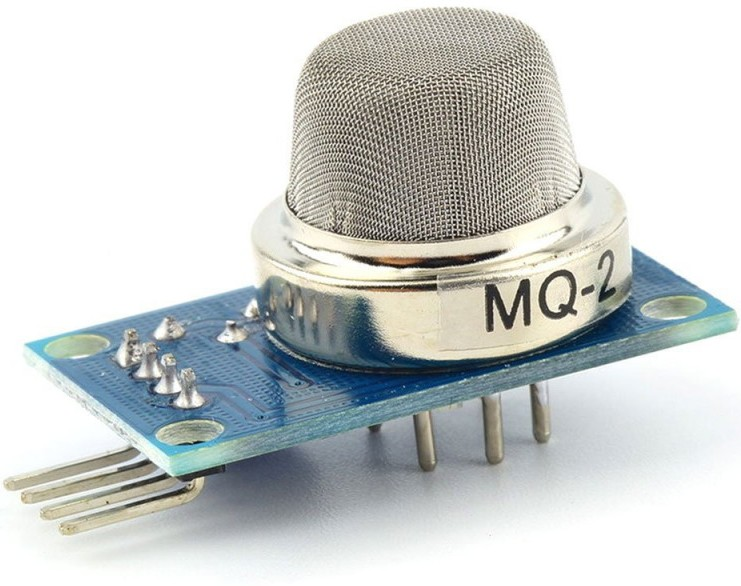
\includegraphics[width=12cm,height=7cm]{figures/mq-2.jpg}
\caption{\label{img37} MQ-2 Gas Sensor}
\end{figure}

\begin{table}[!ht]
\centering
\begin{tabular}{ |p{1cm}|p{2cm}|p{8cm}|  }
\hline
\multicolumn{3}{|c|}{Pin Configuration} \\
\hline
Pin No: & Pin Name: & Description \\
\hline
1 & Vcc  & This pin powers the module, typically the operating voltage is +5V\\
2 & Ground & Used to connect the module to system ground\\
3 & Digital Out & You can also use this sensor to get digital output from this pin, by setting a threshold value using the potentiometer\\
4 & Analog Out & This pin outputs 0-5V analog voltage based on the intensity of the gas \\
\hline
\end{tabular}
\caption{\label{mq-2pin}Pin Diagram of MQ-2 Sensor}
\end{table}


\begin{figure}[!ht]
\centering
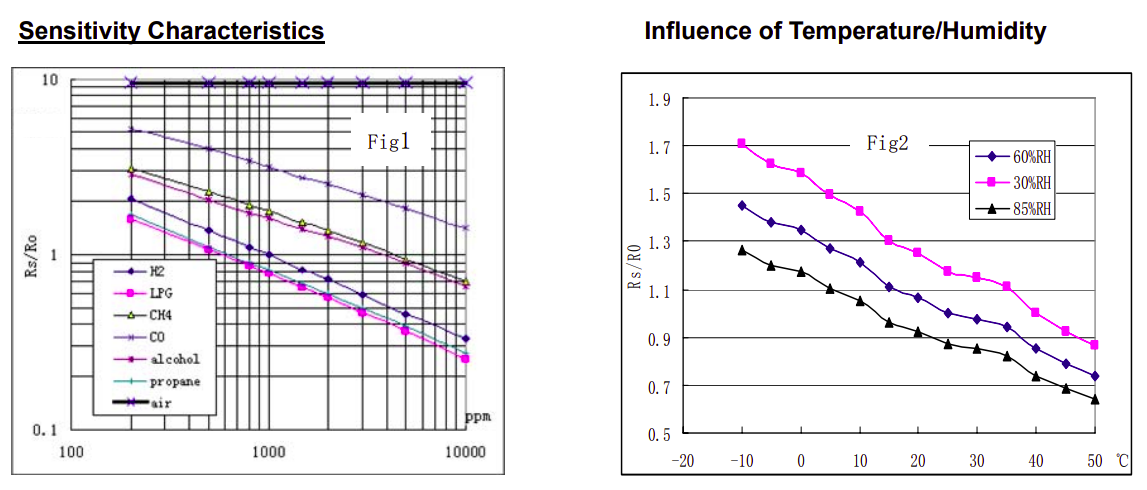
\includegraphics[width=\linewidth]{figures/mq2-datasheet.png}
\caption{\label{img38} MQ-2 Sensor Datasheet}
\end{figure}

\subsection{MQ-7 Carbon Monoxide Sensor}

The MQ-7 carbon monoxide sensor module allows for the sensing of CO concentrations in the air. This module can detect CO gas concentrations from anywhere between 20 and 2000ppm.

 It make detection by method of cycle high and low temperature, and detect CO when low temperature (heated by 1.5V). The sensor’s conductivity is more higher along with the gas concentration rising. When high temperature (heated by 5.0V), it cleans the other gases adsorbed under low temperature. The sensor is highly sensitive and has a quick response time. It uses analogue resistance as an output and is extremely easy to connect with any microcontroller.
 \begin{figure}[!ht]
\centering
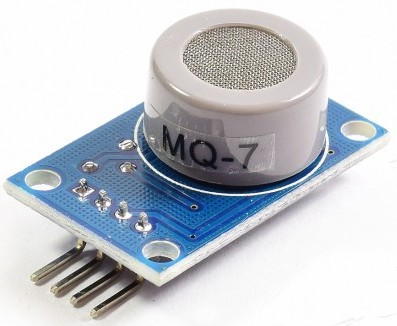
\includegraphics[width=12cm,height=7cm]{figures/mq-7.jpg}
\caption{\label{img39} MQ-7 Carbon Monoxide Sensor}
\end{figure} 
 
 \begin{table}[!ht]
\centering
\begin{tabular}{ |p{1cm}|p{2cm}|p{8cm}|  }
\hline
\multicolumn{3}{|c|}{Pin Configuration} \\
\hline
Pin No: & Pin Name: & Description \\
\hline
1 & Vcc  & This pin powers the module, typically the operating voltage is +5V\\
2 & Ground & Used to connect the module to system ground\\
3 & Digital Out & You can also use this sensor to get digital output from this pin, by setting a threshold value using the potentiometer\\
4 & Analog Out & This pin outputs 0-5V analog voltage based on the intensity of the gas \\
\hline
\end{tabular}
\caption{\label{mq-7pin}Pin Diagram of MQ-7 Sensor}
\end{table}
 
 
 
\begin{figure}[!ht]
\centering
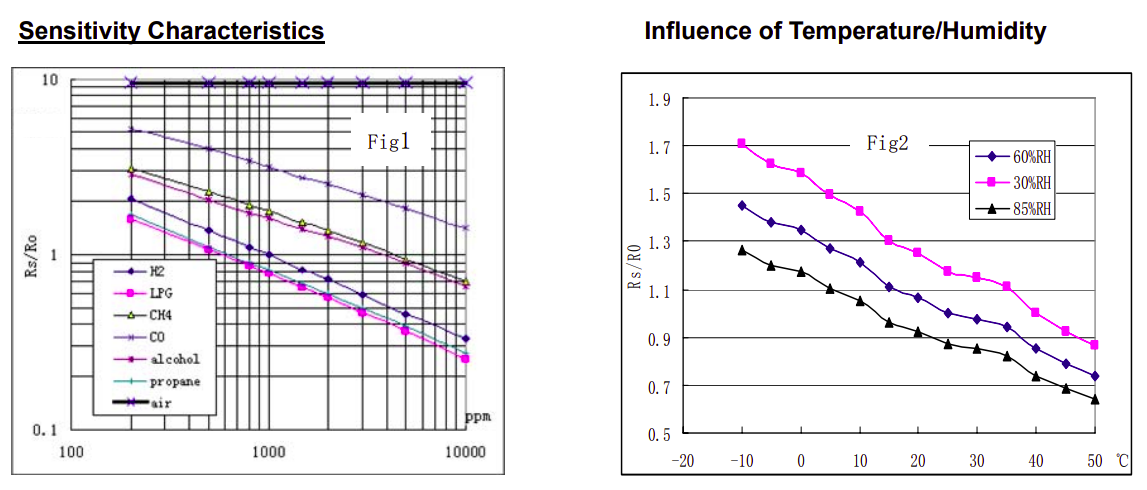
\includegraphics[width=\linewidth]{figures/mq7-datasheet.png}
\caption{\label{img310} MQ-7 Sensor Datasheet}
\end{figure}

\subsection{MQ-135 Air Quality Sensor }

The MQ-135 Gas sensors are used in air quality control equipments and are suitable for detecting or measuring of NH3, NOx, Alcohol, Benzene, Smoke, CO2. The MQ-135 sensor module comes with a Digital Pin which makes this sensor to operate even without a microcontroller and that comes in handy when you are only trying to detect one particular gas.  If you need to measure the gases in PPM the analog pin need to be used. The analog pin is TTL driven and works on 5V and so can be used with most common microcontrollers.

 \begin{figure}[!ht]
\centering
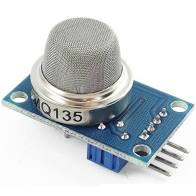
\includegraphics[width=12cm,height=10cm]{figures/mq-135.jpeg}
\caption{\label{img311} MQ-135 Air Quality Sensor}
\end{figure} 
 
 \begin{table}[!ht]
\centering
\begin{tabular}{ |p{1cm}|p{2cm}|p{8cm}|  }
\hline
\multicolumn{3}{|c|}{Pin Configuration} \\
\hline
Pin No: & Pin Name: & Description \\
\hline
1 & Vcc  & This pin powers the module, typically the operating voltage is +5V\\
2 & Ground & Used to connect the module to system ground\\
3 & Digital Out & You can also use this sensor to get digital output from this pin, by setting a threshold value using the potentiometer\\
4 & Analog Out & This pin outputs 0-5V analog voltage based on the intensity of the gas \\
\hline
\end{tabular}
\caption{\label{mq-135pin}Pin Diagram of MQ-135 Sensor}
\end{table}
 
 
 
\begin{figure}[!ht]
\centering
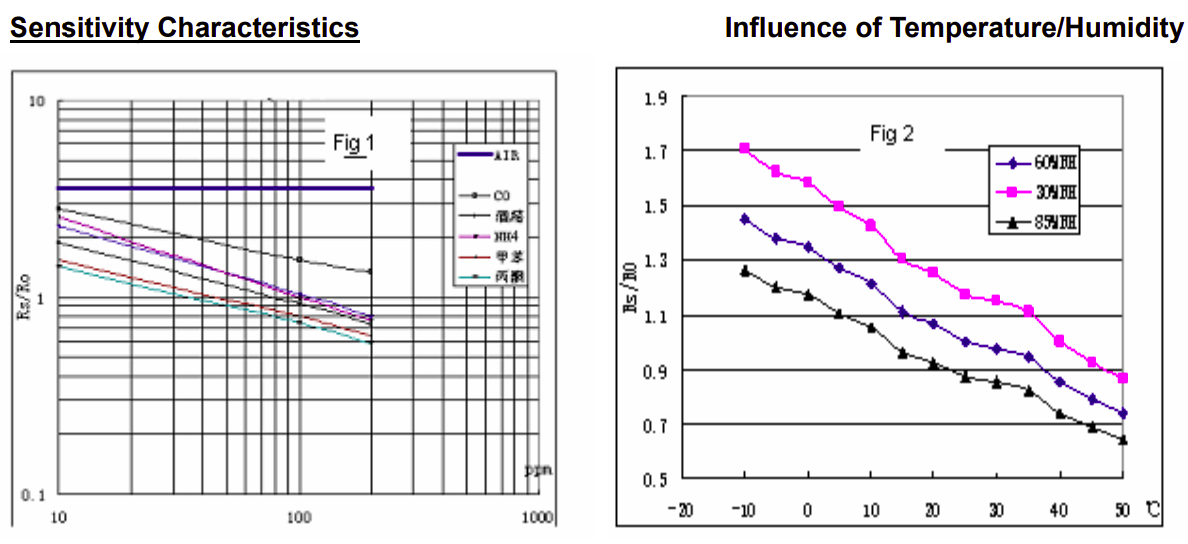
\includegraphics[width=\linewidth]{figures/mq135-datasheet.png}
\caption{\label{img312} MQ-135 Sensor Datasheet}
\end{figure}


\subsection{DHT-11 Temperature \& Humidity Sensor}

The DHT11 is a basic, ultra low-cost digital temperature and humidity sensor. It uses a capacitive humidity sensor and a thermistor to measure the surrounding air, and spits out a digital signal on the data pin (no analog input pins needed). Its fairly simple to use, but requires careful timing to grab data. The only real downside of this sensor is you can only get new data from it once every 2 seconds, so when using our library, sensor readings can be up to 2 seconds old.

\begin{figure}[!ht]
\centering
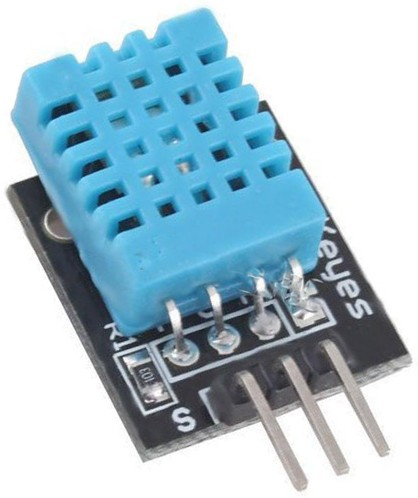
\includegraphics[width=12cm,height=10cm]{figures/dth11}
\caption{\label{img313} DHT-11 Temperature \& Humidity Sensor}
\end{figure}

\begin{table}[!ht]
\centering
\begin{tabular}{ |p{1cm}|p{2cm}|p{8cm}|  }
\hline
\multicolumn{3}{|c|}{Pin Configuration} \\
\hline
Pin No: & Pin Name: & Description \\
\hline
1 & Vcc  & Power supply 3.5V to 5.5V\\
2 & Data & Outputs both Temperature and Humidity through serial Data\\
3 & NC & No Connection and hence not used\\
4 & Ground & Connected to the ground of the circuits \\
\hline
\end{tabular}
\caption{\label{dht-11sensor}Pin Diagram of DHT-11 Sensor}
\end{table}
 
% Research~\cite{silber} in science and \index{technology} has played a vital role in improvising human life at great extent. With the development of instrumentation and computation facilities, research on frontier areas has gone manifold. The discussion on the frontier areas of research in inter- disciplinary subject has always yielded novel ideas and collaborative research. The aim of the conference is to provide a common platform to share and discuss the novel ideas, technologies and research findings to promote interdisciplinary research and to ignite young brains.


% \begin{table}[!ht]
% \centering
% \begin{tabular}{@{}p{10 cm}cccc@{}}\hline
% Research in science and technology & 1 & 2 & 3 & 5 \\
% Research in basic science& 1 & 2 & 3 & 5 \\
% Research in engineering sciences& 1 & 2 & 3 & 5 \\
% \hline
% \end{tabular}
% \caption{\label{data}Table caption 1}
% \end{table}

% Here is the description of Table~\ref{data}. Research in science and technology has played a vital role in improvising human life at great extent. With the development of instrumentation and computation facilities, research on frontier areas has gone manifold. 

% \begin{figure}[!ht]
% \centering
% \includegraphics[scale=0.9]{car1.png}
% \caption{\label{img5} Entity relation ship diagram}
% \end{figure}

% Description of Figure~\ref{img5}. .... 
% Research in science and technology has played a vital role in improvising human life at great extent. With the development of instrumentation and computation facilities, research on frontier areas has gone manifold. 



% \section{Summary}
% ............
